\documentclass[12pt,onecolumn]{article}


\usepackage{xcolor}
\usepackage{graphicx}
\usepackage[top=2cm,bottom=2cm,left=2cm,right=2cm]{geometry}

\title{Unidentified flying object}
\author{Zhang Wei}
\date{29-09-2020}




\begin{document}
\maketitle

\thispagestyle{empty}

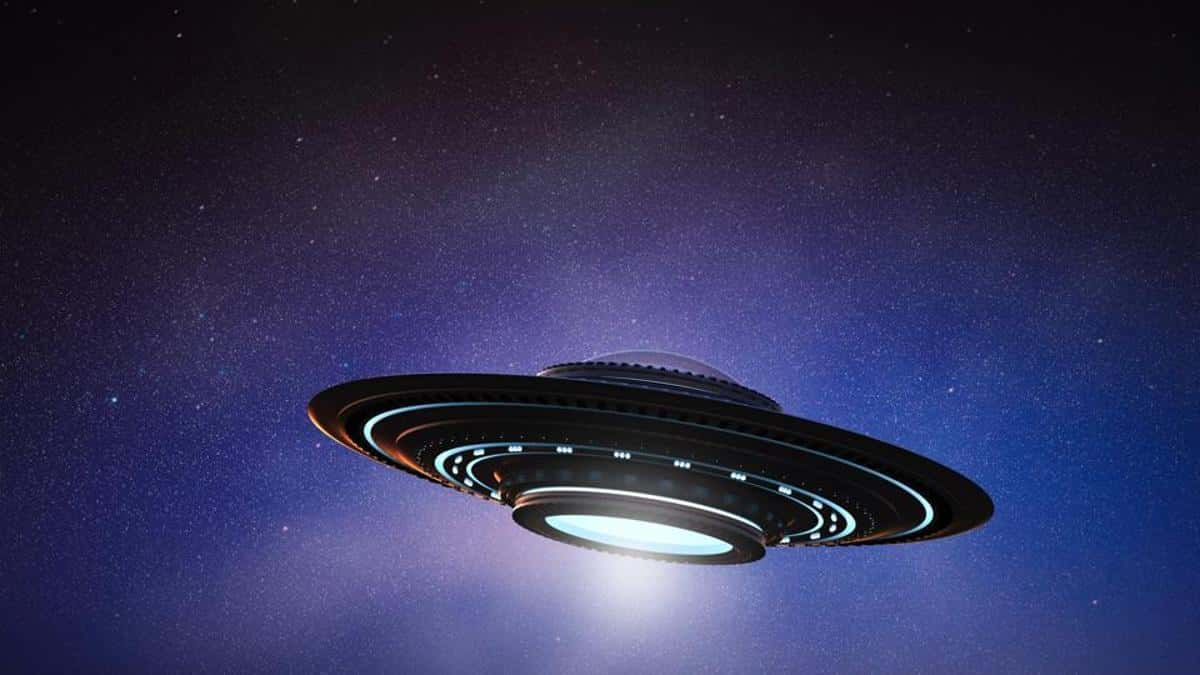
\includegraphics[scale=0.2]{C:/Users/linkeddots/Documents/LaTex-Tutorial/Article Writing/UFO/Image/ufo-in-space.jpg}

\begin{center}
\textcolor{red}{\textbf{Unidentified flying object (UFO)}}, also called flying saucer, any aerial object or optical phenomenon not readily identifiable to the observer. UFOs became a major subject of interest following the development of rocketry after World War II and were thought by some researchers to be intelligent extraterrestrial life visiting Earth.The first well-known UFO sighting occurred in 1947, when businessman Kenneth Arnold claimed to see a group of nine high-speed objects near Mount Rainier in Washington while flying his small plane. Arnold estimated the speed of the crescent-shaped objects as several thousand miles per hour and said they moved like saucers skipping on water.In the newspaper report that followed, it was mistakenly stated that the objects were saucer-shaped, hence the term flying saucer.
\end{center}


\end{document}